\documentclass[11pt,a4paper]{article}

% === PACKAGES ===
\usepackage[utf8]{inputenc}
\usepackage[T1]{fontenc}
\usepackage{mathpazo}  % Palatino font
\usepackage{amsmath,amssymb,amsthm}
\usepackage{graphicx}
\usepackage{xcolor}
\usepackage{hyperref}
\usepackage{cleveref}
\usepackage{listings}
\usepackage{tcolorbox}
\usepackage{tikz}
\usetikzlibrary{automata,positioning,arrows.meta}
\usepackage[margin=1in]{geometry}
\usepackage{enumitem}
\usepackage{booktabs}
\usepackage{caption}

% === COLORS ===
\definecolor{emicblue}{RGB}{41,98,255}
\definecolor{emicgreen}{RGB}{0,150,136}
\definecolor{emicgray}{RGB}{245,245,245}
\definecolor{codebg}{RGB}{250,250,250}
\definecolor{theorembg}{RGB}{255,250,240}

% === HYPERREF SETUP ===
\hypersetup{
    colorlinks=true,
    linkcolor=emicblue,
    citecolor=emicgreen,
    urlcolor=emicblue
}

% === LISTINGS SETUP ===
\lstset{
    language=Python,
    basicstyle=\small\ttfamily,
    backgroundcolor=\color{codebg},
    frame=single,
    framerule=0pt,
    xleftmargin=1em,
    xrightmargin=1em,
    breaklines=true,
    showstringspaces=false,
    keywordstyle=\color{emicblue}\bfseries,
    commentstyle=\color{gray}\itshape,
    stringstyle=\color{emicgreen}
}

% === TCOLORBOX ENVIRONMENTS ===
\tcbuselibrary{skins,breakable}

\newtcolorbox{keyidea}[1][]{
    enhanced,
    colback=emicblue!5,
    colframe=emicblue,
    fonttitle=\bfseries,
    title=Key Idea,
    #1
}

\newtcolorbox{intuition}[1][]{
    enhanced,
    colback=purple!5,
    colframe=purple!70!black,
    fonttitle=\bfseries,
    title=Intuition,
    #1
}

\newtcolorbox{example}[1][]{
    enhanced,
    colback=emicgreen!5,
    colframe=emicgreen,
    fonttitle=\bfseries,
    title=Example,
    #1
}

\newtcolorbox{exercise}[1][]{
    enhanced,
    colback=orange!5,
    colframe=orange!80!black,
    fonttitle=\bfseries,
    title=Exercise,
    #1
}

\newtcolorbox{warning}[1][]{
    enhanced,
    colback=red!5,
    colframe=red!70!black,
    fonttitle=\bfseries,
    title=Common Mistake,
    #1
}

\newtcolorbox{theorembox}[1][]{
    enhanced,
    colback=theorembg,
    colframe=orange!60!black,
    fonttitle=\bfseries,
    #1
}

% === THEOREM ENVIRONMENTS ===
\theoremstyle{definition}
\newtheorem{definition}{Definition}[section]
\theoremstyle{plain}
\newtheorem{theorem}{Theorem}[section]
\newtheorem{lemma}[theorem]{Lemma}
\newtheorem{corollary}[theorem]{Corollary}

% === NOTATION ===
\newcommand{\eps}{\varepsilon}
\newcommand{\Cmu}{C_\mu}
\newcommand{\hmu}{h_\mu}
\newcommand{\calS}{\mathcal{S}}
\newcommand{\calA}{\mathcal{A}}
\newcommand{\Past}{\overleftarrow{S}}
\newcommand{\Future}{\overrightarrow{S}}
\newcommand{\past}{\overleftarrow{s}}
\newcommand{\future}{\overrightarrow{s}}
\DeclareMathOperator{\Ent}{H}
\DeclareMathOperator{\MI}{I}

% === TITLE ===
\title{%
    \vspace{-2em}
    {\Large A Practical Guide to}\\[0.5em]
    {\Huge\bfseries Computational Mechanics}\\[0.5em]
    {\large Finding Hidden Structure in Random Processes}
}
\author{%
    John S Azariah\\
    \small University of Technology, Sydney (UTS)\\
    \small\texttt{john.azariah@student.uts.edu.au}
}
\date{January 2026 --- Draft}

\begin{document}

\maketitle

\begin{abstract}
This tutorial provides a comprehensive introduction to Computational Mechanics, the mathematical framework for understanding structure and complexity in stochastic processes. Starting from first principles, we build up to the six fundamental theorems that establish the $\eps$-machine as the unique optimal predictor. We develop both the frequentist construction (via the CSSR algorithm) and the Bayesian perspective (via Dirichlet-multinomial inference). Throughout, we emphasize intuition and worked examples using the \texttt{emic} Python library.
\end{abstract}

\tableofcontents
\newpage

%%%%%%%%%%%%%%%%%%%%%%%%%%%%%%%%%%%%%%%%%%%%%%%%%%%%%%%%%%%%%%%%%%%%%
\part{Foundations}
%%%%%%%%%%%%%%%%%%%%%%%%%%%%%%%%%%%%%%%%%%%%%%%%%%%%%%%%%%%%%%%%%%%%%

% ===================================================================
\section{The Problem: Hidden Patterns in Randomness}
\label{sec:problem}
% ===================================================================

\begin{keyidea}
Even random-looking sequences often contain hidden structure. Computational Mechanics provides a principled way to discover this structure and quantify its complexity.
\end{keyidea}

Consider flipping a fair coin repeatedly. The sequence looks like:
\begin{center}
\texttt{0 1 1 0 1 0 0 1 1 1 0 1 0 0 1 0 1 1 0 0 ...}
\end{center}

Now consider a different rule: ``After a 0, you \emph{must} output a 1. After a 1, flip fairly.'' This generates sequences like:
\begin{center}
\texttt{1 0 1 1 1 0 1 0 1 1 0 1 1 1 0 1 0 1 1 0 ...}
\end{center}

Both sequences look random to the naked eye. But the second has \emph{structure}---it was generated by a two-state machine that ``remembers'' whether the last symbol was 0 or 1.

\begin{quote}
\textbf{The Central Question:} \emph{Given only the observed data, can we discover this hidden structure? And can we do so optimally---finding the simplest model that captures all the predictive information?}
\end{quote}

Computational Mechanics answers both questions affirmatively. It provides:
\begin{enumerate}
    \item A \textbf{definition} of what ``structure'' means (causal states)
    \item A \textbf{construction} of the minimal predictive model ($\eps$-machine)
    \item \textbf{Proofs} that this model is optimal and unique
    \item \textbf{Algorithms} to infer it from data
    \item \textbf{Measures} to quantify the structure ($\Cmu$, $\hmu$, $E$)
\end{enumerate}

This tutorial uses the \texttt{emic} Python library\footnote{Available at \url{https://github.com/johnazariah/emic}. The online documentation at \url{https://johnazariah.github.io/emic/} includes additional algorithm deep dives and practical guides for working with real data.} for all examples. Let's begin by understanding why this matters.

\subsection{Why Does This Matter?}

Structure detection appears across science:
\begin{itemize}
    \item \textbf{Physics}: Finding order parameters in phase transitions
    \item \textbf{Neuroscience}: Discovering neural codes in spike trains
    \item \textbf{Finance}: Detecting regimes in market behavior
    \item \textbf{Biology}: Understanding gene regulatory dynamics
    \item \textbf{Language}: Modeling statistical structure in text
\end{itemize}

In each case, we observe a stream of symbols and want to infer the hidden process that generated them.

% ===================================================================
\section{Probability Refresher}
\label{sec:probability}
% ===================================================================

Before diving into Computational Mechanics, let's establish the probability concepts we'll need.

\subsection{Random Variables and Distributions}

A \textbf{random variable} $X$ assigns outcomes to events. A \textbf{probability distribution} $P(X = x)$ tells us how likely each outcome is.

\begin{example}[title=Biased Coin]
A coin lands heads with probability $\theta = 0.7$:
\begin{align*}
    P(X = \text{heads}) &= 0.7 \\
    P(X = \text{tails}) &= 0.3
\end{align*}
\end{example}

\textbf{Key rule}: All probabilities sum to 1.

\subsection{Conditional Probability}

The \textbf{conditional probability} $P(X | Y)$ is the probability of $X$ \emph{given that we know} $Y$:
\begin{equation}
    P(X = x | Y = y) = \frac{P(X = x, Y = y)}{P(Y = y)}
\end{equation}

\begin{intuition}
Conditioning is like filtering. If we know $Y = y$, we restrict our attention to outcomes where $Y = y$ occurred.
\end{intuition}

\subsection{Independence}

Two random variables are \textbf{independent} if knowing one tells you nothing about the other:
\begin{equation}
    P(X, Y) = P(X) \cdot P(Y) \quad \Leftrightarrow \quad P(X|Y) = P(X)
\end{equation}

% ===================================================================
\section{Information Theory Essentials}
\label{sec:information-theory}
% ===================================================================

Information theory, developed by Claude Shannon in 1948~\cite{shannon1948mathematical}, provides the mathematical language for quantifying uncertainty and information. For a comprehensive treatment, see Cover and Thomas~\cite{cover2006elements}.

\subsection{Entropy: Quantifying Uncertainty}

\begin{definition}[Shannon Entropy]
The \textbf{entropy} of a random variable $X$ is:
\begin{equation}
    \Ent[X] = -\sum_{x} P(x) \log_2 P(x)
\end{equation}
measured in \textbf{bits}.
\end{definition}

\begin{intuition}
Entropy measures \emph{surprise}. If an event has probability $p$, its surprise is $-\log_2 p$ bits. Entropy is the \emph{average} surprise.
\end{intuition}

\begin{example}[title=Entropy of a Coin]
\textbf{Fair coin} ($p = 0.5$):
\[
    \Ent = -0.5 \log_2 0.5 - 0.5 \log_2 0.5 = 1 \text{ bit}
\]
\textbf{Biased coin} ($p = 0.9$):
\[
    \Ent = -0.9 \log_2 0.9 - 0.1 \log_2 0.1 \approx 0.47 \text{ bits}
\]
Maximum entropy = maximum uncertainty = fair coin.
\end{example}

\subsection{Joint and Conditional Entropy}

\textbf{Joint entropy} measures uncertainty about both $X$ and $Y$:
\begin{equation}
    \Ent[X, Y] = -\sum_{x,y} P(x, y) \log_2 P(x, y)
\end{equation}

\textbf{Conditional entropy} measures remaining uncertainty about $X$ after learning $Y$:
\begin{equation}
    \Ent[X | Y] = \Ent[X, Y] - \Ent[Y]
\end{equation}

\begin{keyidea}
Conditioning reduces entropy (or keeps it the same): $\Ent[X|Y] \leq \Ent[X]$.
\end{keyidea}

\subsection{Mutual Information}

\textbf{Mutual information} measures how much knowing $Y$ tells us about $X$:
\begin{equation}
    \MI(X; Y) = \Ent[X] - \Ent[X|Y] = \Ent[Y] - \Ent[Y|X]
\end{equation}

\begin{intuition}
$\MI(X; Y)$ is the reduction in uncertainty about $X$ from learning $Y$. It's symmetric: $X$ tells us as much about $Y$ as $Y$ tells us about $X$.
\end{intuition}

% ===================================================================
\section{Stochastic Processes}
\label{sec:processes}
% ===================================================================

\begin{definition}[Stochastic Process]
A \textbf{stochastic process} is a sequence of random variables $\ldots, X_{-1}, X_0, X_1, X_2, \ldots$ taking values in an alphabet $\calA$.
\end{definition}

We denote:
\begin{itemize}
    \item $\Past = \ldots X_{-2} X_{-1}$: the semi-infinite \textbf{past}
    \item $\Future = X_0 X_1 X_2 \ldots$: the semi-infinite \textbf{future}
    \item $X_0^{L-1} = X_0 X_1 \ldots X_{L-1}$: a block of length $L$
\end{itemize}

\begin{definition}[Stationarity]
A process is \textbf{stationary} if its statistics don't change over time:
\[
    P(X_t^{t+L} = s) = P(X_0^L = s) \quad \text{for all } t, L
\]
\end{definition}

\subsection{The Entropy Rate}

For a stationary process, the \textbf{entropy rate} is the asymptotic per-symbol entropy:
\begin{equation}
    \hmu = \lim_{L \to \infty} \frac{1}{L} \Ent[X_0^{L-1}] = \lim_{L \to \infty} \Ent[X_L | X_0^{L-1}]
\end{equation}

\begin{intuition}
$\hmu$ measures the \emph{irreducible randomness} per symbol---the uncertainty that remains even after seeing arbitrarily long histories.
\end{intuition}

\subsection{Excess Entropy}

The \textbf{excess entropy}~\cite{grassberger1986toward} is the mutual information between past and future:
\begin{equation}
    E = \MI(\Past; \Future)
\end{equation}

\begin{intuition}
$E$ measures how much the past tells us about the future---the ``apparent memory'' visible in the data.
\end{intuition}

%%%%%%%%%%%%%%%%%%%%%%%%%%%%%%%%%%%%%%%%%%%%%%%%%%%%%%%%%%%%%%%%%%%%%
\part{\texorpdfstring{Causal States and the $\eps$-Machine}{Causal States and the Epsilon-Machine}}
%%%%%%%%%%%%%%%%%%%%%%%%%%%%%%%%%%%%%%%%%%%%%%%%%%%%%%%%%%%%%%%%%%%%%

The concepts in this section were developed by Crutchfield and Young~\cite{crutchfield1989inferring} and formalized fully by Shalizi and Crutchfield~\cite{shalizi2001computational}.

% ===================================================================
\section{The Key Insight: Prediction-Equivalent Histories}
\label{sec:key-insight}
% ===================================================================

Here's the fundamental insight of Computational Mechanics:

\begin{keyidea}
Two histories are ``the same'' if they make the same predictions about the future.
\end{keyidea}

Consider predicting the next symbol of a process. The full history $\past = \ldots x_{-3} x_{-2} x_{-1}$ determines the conditional distribution $P(\Future | \Past = \past)$.

But do we really need the \emph{entire} history? Often, different histories lead to the same predictions.

\begin{example}[title=Golden Mean Process]
In the Golden Mean process, the histories ``$\ldots 1 1 0 1$'' and ``$\ldots 0 1 0 1$'' both end in 1. Since the rule is ``after 1, flip fairly,'' both histories predict:
\[
    P(\text{next} = 0) = 0.5, \quad P(\text{next} = 1) = 0.5
\]
They're \emph{prediction-equivalent}---we can group them together!
\end{example}

% ===================================================================
\section{Causal States: The Formal Definition}
\label{sec:causal-states}
% ===================================================================

\begin{definition}[Causal Equivalence]
\label{def:causal-equiv}
Two histories $\past, \past'$ are \textbf{causally equivalent}, written $\past \sim_\eps \past'$, if they have the same conditional distribution over all futures:
\begin{equation}
    P(\Future | \Past = \past) = P(\Future | \Past = \past')
\end{equation}
\end{definition}

This is clearly an equivalence relation (reflexive, symmetric, transitive).

\begin{definition}[Causal States]
\label{def:causal-state}
The \textbf{causal states} $\calS$ are the equivalence classes under $\sim_\eps$:
\begin{equation}
    \calS = \{\text{histories}\} / \sim_\eps
\end{equation}
The function $\epsilon: \{\text{histories}\} \to \calS$ maps each history to its causal state.
\end{definition}

\begin{intuition}
A causal state is a ``sufficient summary'' of the past. It retains exactly the information needed for optimal prediction---no more, no less.
\end{intuition}

\subsection{Morphs: The Predictive Signature}

Each causal state $\sigma \in \calS$ has an associated \textbf{morph}---the conditional distribution over futures:
\begin{equation}
    P(\Future | \epsilon(\past) = \sigma) = P(\Future | \Past = \past) \quad \text{for any } \past \in \sigma
\end{equation}

Different causal states have different morphs. The morph is what makes each state ``who it is.''

% ===================================================================
\section{The \texorpdfstring{$\eps$}{ε}-Machine}
\label{sec:epsilon-machine}
% ===================================================================

\begin{definition}[$\eps$-Machine]
The \textbf{$\eps$-machine} of a process is the tuple $\{\calS, \calA, T, \pi\}$ where:
\begin{itemize}
    \item $\calS$ = the causal states
    \item $\calA$ = the alphabet
    \item $T^{(x)}_{\sigma \sigma'}$ = probability of transitioning from $\sigma$ to $\sigma'$ while emitting symbol $x$
    \item $\pi$ = the stationary distribution over states
\end{itemize}
\end{definition}

\begin{center}
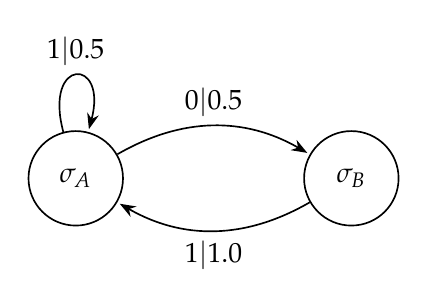
\begin{tikzpicture}[->,>=Stealth,shorten >=1pt,auto,node distance=3.5cm,
                    semithick,every state/.style={minimum size=1.2cm}]
    \node[state] (A) {$\sigma_A$};
    \node[state] (B) [right of=A] {$\sigma_B$};

    \path (A) edge [loop above] node {$1|0.5$} (A)
          (A) edge [bend left]  node {$0|0.5$} (B)
          (B) edge [bend left]  node {$1|1.0$} (A);
\end{tikzpicture}
\captionof{figure}{The $\eps$-machine for the Golden Mean process. Edge labels show ``symbol$|$probability.''}
\end{center}

\subsection{Unifilarity: A Key Property}

\begin{definition}[Unifilarity]
An $\eps$-machine is \textbf{unifilar} if each state-symbol pair determines a unique next state. That is, if we're in state $\sigma$ and emit symbol $x$, we know exactly which state comes next.
\end{definition}

\begin{lemma}
The $\eps$-machine is always unifilar.
\end{lemma}

\begin{proof}[Proof Sketch]
If history $\past$ leads to state $\sigma$, then history $\past x$ leads to a specific state $\sigma'$ that depends only on $\sigma$ and $x$, not on the specific history $\past$.
\end{proof}

\begin{keyidea}
Unifilarity means we can track the current state by observing the output sequence. No hidden randomness in the state transitions---all randomness is in choosing \emph{which symbol} to emit.
\end{keyidea}

%%%%%%%%%%%%%%%%%%%%%%%%%%%%%%%%%%%%%%%%%%%%%%%%%%%%%%%%%%%%%%%%%%%%%
\part{The Six Theorems}
%%%%%%%%%%%%%%%%%%%%%%%%%%%%%%%%%%%%%%%%%%%%%%%%%%%%%%%%%%%%%%%%%%%%%

The power of Computational Mechanics comes from six theorems established by Shalizi and Crutchfield~\cite{shalizi2001computational} that together prove the $\eps$-machine is the unique optimal predictor. These theorems are not merely mathematical curiosities---they provide the theoretical foundation for why $\eps$-machines are the ``right'' way to represent process structure.

% ===================================================================
\section{Theorem 1: Prescience (Causal States Predict Optimally)}
\label{sec:theorem-prescience}
% ===================================================================

\subsection{Background: The Prediction Problem}

Given a stochastic process $\{X_t\}$, suppose we've observed a history $\past = \ldots x_{-2} x_{-1} x_0$ and want to predict the future $\future = x_1 x_2 \ldots$. The fundamental question: \emph{what should we remember about the past to make optimal predictions?}

Clearly, knowing the entire history $\past$ gives the best possible prediction. But histories are infinite---we can't store them all. We need a \emph{finite representation} that captures ``what matters'' for prediction.

\subsection{Notation and Setup}

\paragraph{Key symbols.}
\begin{itemize}[nosep]
    \item $\Ent[\cdot]$ --- Shannon entropy~\cite{shannon1948mathematical}, measuring uncertainty in bits
    \item $\Ent[Y | X]$ --- conditional entropy: average uncertainty in $Y$ given knowledge of $X$
    \item $\Future^L = X_1 X_2 \ldots X_L$ --- the next $L$ symbols of the future
    \item $R : \Past \to \mathcal{R}$ --- any function that maps histories to a finite set of ``states''
    \item $\calS$ --- the set of causal states (our special partition based on predictive equivalence)
\end{itemize}

\paragraph{What is a ``partition''?} A partition $R$ groups histories into equivalence classes. Given history $\past$, we assign it to state $R(\past)$. Different histories may map to the same state. The key question: which partition gives the best predictions?

\subsection{The Theorem}

\begin{theorembox}[title=Theorem 1: Prescience~\cite{shalizi2001computational}]
\begin{theorem}[Causal States are Maximally Prescient]
\label{thm:prescience}
For any partition of histories $R$, and any prediction horizon $L$:
\begin{equation}
    \Ent[\Future^L | R] \geq \Ent[\Future^L | \calS]
\end{equation}
where $\calS$ denotes the causal state partition.
\end{theorem}
\end{theorembox}

\paragraph{Reading the inequality.}
\begin{itemize}[nosep]
    \item Left side: ``uncertainty about the next $L$ symbols, given that we know which class $R$ assigns to our history''
    \item Right side: ``uncertainty about the next $L$ symbols, given that we know the causal state''
    \item The inequality: causal states leave us with \emph{less or equal} uncertainty---they never predict worse than any alternative
\end{itemize}

\subsection{Proof Walkthrough}

The proof proceeds in three steps:

\paragraph{Step 1: The full history is optimal.}
By the data processing inequality~\cite{cover2006elements}, conditioning on more information never increases entropy:
\begin{equation}
    \Ent[\Future^L | \Past] \leq \Ent[\Future^L | R(\Past)]
\end{equation}
for any function $R$. The full history $\Past$ gives the best possible prediction.

\paragraph{Step 2: Causal states preserve predictive information.}
By the \emph{definition} of causal states (Definition~\ref{def:causal-state}), two histories $\past$ and $\past'$ are in the same causal state if and only if they have identical conditional distributions over futures:
\begin{equation}
    P(\Future | \past) = P(\Future | \past')
\end{equation}
This means knowing the causal state gives exactly the same predictive distribution as knowing the full history:
\begin{equation}
    \Ent[\Future^L | \calS] = \Ent[\Future^L | \Past]
\end{equation}

\paragraph{Step 3: Any other partition is at least as uncertain.}
Any other partition $R$ either:
\begin{itemize}[nosep]
    \item Is a \emph{refinement} of $\calS$ (distinguishes histories that $\calS$ groups together), in which case it matches $\calS$'s predictions, or
    \item Is \emph{coarser} than $\calS$ (groups histories that $\calS$ distinguishes), in which case it loses predictive information
\end{itemize}
In either case, $\Ent[\Future^L | R] \geq \Ent[\Future^L | \calS]$. \qed

\begin{intuition}
No matter how you group histories, you can't predict the future better than by using causal states. The causal states are \emph{sufficient statistics} for prediction---they capture everything predictively relevant about the past.
\end{intuition}

\begin{corollary}[Sufficient Statistics]
The causal states $\calS$ are sufficient statistics for predicting $\Future$. In the language of statistics, $\Past \to \calS \to \Future$ forms a Markov chain.
\end{corollary}

% ===================================================================
\section{Theorem 2: Minimality (Simplest Prescient Representation)}
\label{sec:theorem-minimality}
% ===================================================================

\subsection{The Compression Problem}

Theorem~\ref{thm:prescience} tells us causal states predict optimally---but are they the \emph{simplest} way to achieve optimal prediction? Perhaps there's a more compact representation that predicts just as well?

This is where Theorem 2 comes in: it shows that among all optimal predictors, causal states use the \emph{least memory}.

\subsection{Notation and Setup}

\paragraph{Key symbols.}
\begin{itemize}[nosep]
    \item $\hat{R}$ --- any alternative representation (partition) of histories
    \item $\Ent[R]$ --- the entropy of the state distribution: $\Ent[R] = -\sum_r P(R=r) \log_2 P(R=r)$
    \item $\Cmu \equiv \Ent[\calS]$ --- statistical complexity~\cite{crutchfield1989inferring}, the entropy of the causal state distribution
    \item ``$\hat{R}$ is prescient'' --- means $\Ent[\Future^L | \hat{R}] = \Ent[\Future^L | \calS]$ for all $L$
\end{itemize}

\paragraph{What does $\Ent[R]$ measure?} The entropy $\Ent[R]$ quantifies the ``size'' of representation $R$ in an information-theoretic sense. It measures how many bits we need on average to specify which state we're in. A representation with many equally-likely states has high entropy; one dominated by a single state has low entropy.

\subsection{The Theorem}

\begin{theorembox}[title=Theorem 2: Minimality~\cite{shalizi2001computational}]
\begin{theorem}[Causal States are Minimal]
\label{thm:minimality}
Among all representations $\hat{R}$ that are as prescient as causal states:
\begin{equation}
    \Ent[\hat{R}] \geq \Ent[\calS] = \Cmu
\end{equation}
\end{theorem}
\end{theorembox}

\paragraph{Reading the inequality.} If $\hat{R}$ predicts as well as causal states, then $\hat{R}$ must use at least as much memory (measured by entropy) as causal states. You cannot achieve optimal prediction with a simpler representation.

\subsection{Proof Walkthrough}

The proof uses a fundamental result from information theory.

\paragraph{Step 1: Set up the information flow.}
Consider the chain $\Past \to \hat{R} \to \Future$. If $\hat{R}$ is prescient (predicts as well as knowing the full past), then by the data processing inequality~\cite{cover2006elements}:
\begin{equation}
    \MI[\Past; \Future] = \MI[\hat{R}; \Future]
\end{equation}
where $\MI$ denotes mutual information. The representation $\hat{R}$ captures \emph{all} the predictive information in the past.

\paragraph{Step 2: Apply the information-theoretic identity.}
The mutual information satisfies:
\begin{equation}
    \MI[\hat{R}; \Future] \leq \Ent[\hat{R}]
\end{equation}
with equality only when $\hat{R}$ is a deterministic function of $\Future$ (which is generally not the case).

\paragraph{Step 3: Causal states achieve the bound.}
Causal states are defined as the \emph{minimal} sufficient statistics for prediction. They achieve:
\begin{equation}
    \Ent[\calS] = \Cmu = \min_{\hat{R} \text{ prescient}} \Ent[\hat{R}]
\end{equation}
Any other prescient $\hat{R}$ must either match this entropy or exceed it. \qed

\begin{intuition}
If you want optimal prediction, you can't do it with a simpler representation than causal states. The $\eps$-machine has the smallest ``memory footprint'' among all optimal predictors.
\end{intuition}

\paragraph{Why this matters.} This is where \emph{Occam's Razor becomes a theorem}! We often invoke parsimony as a heuristic---prefer simpler models. Theorem 2 proves that for prediction, the simplest optimal model is unique and well-defined: it's the $\eps$-machine.

% ===================================================================
\section{Theorem 3: Uniqueness}
\label{sec:theorem-uniqueness}
% ===================================================================

\subsection{The Identification Problem}

We've established that causal states are:
\begin{enumerate}[nosep]
    \item \textbf{Prescient}: They predict as well as knowing the full history (Theorem~\ref{thm:prescience})
    \item \textbf{Minimal}: No simpler representation predicts as well (Theorem~\ref{thm:minimality})
\end{enumerate}

But could there be \emph{multiple} representations that are both optimal and minimal? Perhaps different constructions lead to equally good but structurally different models?

Theorem 3 answers decisively: \emph{no}. The $\eps$-machine is unique.

\subsection{Notation and Setup}

\paragraph{Key concepts.}
\begin{itemize}[nosep]
    \item ``$\hat{R}$ is prescient'' --- $\hat{R}$ predicts as well as causal states for all horizons
    \item ``$\hat{R}$ is minimal'' --- $\Ent[\hat{R}] = \Cmu$ (achieves the lower bound from Theorem~\ref{thm:minimality})
    \item ``Equivalent up to relabeling'' --- there exists a bijection $\phi: \hat{\mathcal{R}} \to \calS$ such that $\phi(\hat{R}(\past)) = \calS(\past)$ for all histories $\past$
\end{itemize}

\subsection{The Theorem}

\begin{theorembox}[title=Theorem 3: Uniqueness~\cite{shalizi2001computational}]
\begin{theorem}[Causal States are Unique]
\label{thm:uniqueness}
If $\hat{R}$ is prescient and $\Ent[\hat{R}] = \Cmu$, then $\hat{R}$ is equivalent to $\calS$ up to relabeling.
\end{theorem}
\end{theorembox}

\subsection{Proof Walkthrough}

The proof shows that any optimal-minimal representation must be isomorphic to causal states.

\paragraph{Step 1: Prescience implies refinement.}
If $\hat{R}$ is prescient, it must distinguish histories that have different predictive futures. Since causal states are defined by predictive equivalence, $\hat{R}$ must be at least as fine as $\calS$---it cannot merge histories that $\calS$ separates.

Formally: if $\calS(\past) \neq \calS(\past')$, then $\hat{R}(\past) \neq \hat{R}(\past')$.

\paragraph{Step 2: Minimality implies no finer than $\calS$.}
If $\hat{R}$ is finer than $\calS$ (distinguishes histories that $\calS$ groups), then $\Ent[\hat{R}] > \Ent[\calS] = \Cmu$. But we assumed $\Ent[\hat{R}] = \Cmu$.

Contradiction. So $\hat{R}$ cannot be finer than $\calS$.

\paragraph{Step 3: Combine to get equality.}
From Steps 1 and 2: $\hat{R}$ is at least as fine as $\calS$, but not finer. Therefore $\hat{R}$ and $\calS$ define the same partition, possibly with different state labels. \qed

\begin{intuition}
There's only one way to be both optimal and minimal. The $\eps$-machine is not just \emph{an} optimal predictor---it's \emph{the} optimal predictor. Any other optimal-minimal model is the $\eps$-machine in disguise.
\end{intuition}

\paragraph{The ``canonical model'' property.} Uniqueness is crucial for interpretation. When we infer an $\eps$-machine from data, we're not finding one of many possible models---we're recovering \emph{the} intrinsic structure of the process. This justifies calling the $\eps$-machine the ``canonical'' representation.

% ===================================================================
\section{Theorem 4: Minimal Stochasticity}
\label{sec:theorem-stochasticity}
% ===================================================================

\subsection{The Transition Entropy Problem}

Theorems 1--3 establish that causal states are the unique optimal-minimal representation. But there's another property we might desire: \emph{predictable dynamics}.

Given that we're in state $\sigma$, how uncertain are we about the \emph{next} state $\sigma'$? Ideally, we'd like the state evolution to be as deterministic as possible---randomness should come from the symbols, not from hidden state transitions.

\subsection{Notation and Setup}

\paragraph{Key symbols.}
\begin{itemize}[nosep]
    \item $\calS$ --- the current causal state
    \item $\calS'$ --- the causal state at the next time step (after observing symbol $X$)
    \item $\Ent[\calS' | \calS]$ --- transition entropy: uncertainty about the next state given the current state
    \item $\Ent[\calS' | \calS, X]$ --- uncertainty about the next state given current state \emph{and} the emitted symbol
\end{itemize}

\paragraph{Unifilarity revisited.} Recall that $\eps$-machines are \emph{unifilar}: given the current state $\sigma$ and the next symbol $x$, the next state $\sigma'$ is determined uniquely. This means $\Ent[\calS' | \calS, X] = 0$---zero uncertainty once we know the symbol.

But $\Ent[\calS' | \calS]$ is generally nonzero, because we don't know which symbol will be emitted.

\subsection{The Theorem}

\begin{theorembox}[title=Theorem 4: Minimal Stochasticity~\cite{shalizi2001computational}]
\begin{theorem}[$\eps$-Machines are Minimally Stochastic]
\label{thm:stochasticity}
For all prescient representations $\hat{R}$:
\begin{equation}
    \Ent[\hat{R}' | \hat{R}] \geq \Ent[\calS' | \calS]
\end{equation}
where $\calS'$ and $\hat{R}'$ denote the next-step states.
\end{theorem}
\end{theorembox}

\paragraph{Reading the inequality.} The left side is the transition entropy for representation $\hat{R}$. The right side is the transition entropy for causal states. The inequality says: no prescient representation has more deterministic dynamics than the $\eps$-machine.

\subsection{Proof Walkthrough}

\paragraph{Step 1: Decompose transition entropy.}
For any representation $\hat{R}$:
\begin{equation}
    \Ent[\hat{R}' | \hat{R}] = \Ent[\hat{R}' | \hat{R}, X] + \MI[\hat{R}'; X | \hat{R}]
\end{equation}
The first term is the ``internal noise''---randomness in transitions not explained by the symbol. The second term is predictable from $X$.

\paragraph{Step 2: Unifilarity minimizes internal noise.}
For the $\eps$-machine, unifilarity gives $\Ent[\calS' | \calS, X] = 0$. The internal noise vanishes completely.

For a non-unifilar representation, the same symbol might lead to different next states---so $\Ent[\hat{R}' | \hat{R}, X] > 0$.

\paragraph{Step 3: Combine the bounds.}
Since $\Ent[\hat{R}' | \hat{R}, X] \geq 0 = \Ent[\calS' | \calS, X]$, and prescient representations preserve the predictive information, we get the inequality. \qed

\begin{intuition}
The transitions between causal states are as deterministic as possible. All randomness in the $\eps$-machine comes from symbol selection, not from hidden state dynamics. There's no ``extra'' noise hiding in the state transitions.
\end{intuition}

\paragraph{Connection to hidden Markov models.} Standard HMMs can have stochastic hidden-to-hidden transitions (even given the observation). The $\eps$-machine's unifilarity property eliminates this source of uncertainty, making it a ``maximally observable'' HMM~\cite{rabiner1989tutorial}.

% ===================================================================
\section{Theorem 5: The Complexity Bound}
\label{sec:theorem-bound}
% ===================================================================

\subsection{Two Measures of Memory}

Theorems 1--4 characterize the $\eps$-machine's optimality properties. Theorems 5 and 6 relate the statistical complexity $\Cmu$ to other information-theoretic quantities, revealing deep connections.

Theorem 5 relates $\Cmu$ to the \emph{excess entropy} $E$---a measure of ``apparent memory'' that can be estimated directly from time series data.

\subsection{Notation and Setup}

\paragraph{Key quantities.}
\begin{itemize}[nosep]
    \item $E \equiv \MI[\Past; \Future]$ --- the \textbf{excess entropy}~\cite{grassberger1986toward}, also called ``effective measure complexity''
    \item $\MI[X; Y] = \Ent[X] - \Ent[X|Y]$ --- mutual information between $X$ and $Y$
    \item $\Cmu \equiv \Ent[\calS]$ --- statistical complexity, the entropy of causal states
    \item $\Ent[\calS | \Future]$ --- residual uncertainty about the current state even knowing the entire future
\end{itemize}

\paragraph{What does excess entropy measure?}
$E = \MI[\Past; \Future]$ quantifies how much the past tells you about the future, summed over all horizons. It measures the \emph{total correlation} between past and future---the ``amount of mutual prediction'' possible.

Crucially, $E$ can be estimated from data without knowing the $\eps$-machine structure, via:
\begin{equation}
    E = \lim_{L \to \infty} \left[ \Ent[X_1^L] - L \cdot \hmu \right]
\end{equation}
where $\Ent[X_1^L]$ is the block entropy of $L$-symbol sequences.

\paragraph{What does $\Cmu$ measure?}
$\Cmu = \Ent[\calS]$ is the entropy of the causal state distribution---the average number of bits needed to specify the current state. It measures the ``true memory'' that the process uses internally.

\subsection{The Theorem}

\begin{theorembox}[title=Theorem 5: The Bound~\cite{shalizi2001computational}]
\begin{theorem}[Excess Entropy Bound]
\label{thm:bound}
The statistical complexity bounds the excess entropy:
\begin{equation}
    E \leq \Cmu
\end{equation}
with equality if and only if $\Ent[\calS | \Future] = 0$.
\end{theorem}
\end{theorembox}

\paragraph{Reading the inequality.} The ``apparent memory'' (visible in correlations) is always less than or equal to the ``true memory'' (stored in causal states). Some structure may be hidden!

\subsection{Proof Walkthrough}

\paragraph{Step 1: Express $E$ in terms of states.}
Since causal states are sufficient statistics for prediction:
\begin{equation}
    E = \MI[\Past; \Future] = \MI[\calS; \Future]
\end{equation}
The past-future mutual information equals the state-future mutual information.

\paragraph{Step 2: Use the mutual information bound.}
By a standard identity:
\begin{equation}
    \MI[\calS; \Future] = \Ent[\calS] - \Ent[\calS | \Future]
\end{equation}
Since entropy is nonnegative:
\begin{equation}
    \MI[\calS; \Future] \leq \Ent[\calS] = \Cmu
\end{equation}
with equality iff $\Ent[\calS | \Future] = 0$.

\paragraph{Step 3: Interpret the gap.}
The quantity $\chi \equiv \Cmu - E = \Ent[\calS | \Future]$ is called the \textbf{crypticity}~\cite{james2011anatomy}. It measures how much of the process's internal memory is \emph{not} reflected in past-future correlations---``hidden'' structure that doesn't affect correlations but is still needed for optimal prediction. \qed

\begin{intuition}
The ``apparent memory'' $E$ (visible in correlations) is always less than or equal to the ``true memory'' $\Cmu$ (stored in causal states). The gap is \emph{crypticity}---structure hidden from correlation analysis.
\end{intuition}

\begin{example}[title=When $E < \Cmu$: Cryptic Processes]
Consider a process that ``remembers'' information for a long time before using it. The current state affects the distant future but not the immediate future. Standard correlation measures (which focus on nearby time points) may miss this structure, giving $E < \Cmu$.

A concrete example: a counter that increments silently for 1000 steps, then resets with a special symbol. The state (counter value) is highly structured ($\Cmu$ is large), but consecutive symbols are nearly independent ($E$ is small).
\end{example}

\paragraph{Practical implication.} When analyzing data, $E$ gives a \emph{lower bound} on the process's true complexity $\Cmu$. If you find $E = 2$ bits, you know the process has \emph{at least} 2 bits of memory---possibly much more.

% ===================================================================
\section{Theorem 6: The Control Theorem}
\label{sec:theorem-control}
% ===================================================================

\subsection{Memory and Predictability}

The final theorem relates the statistical complexity to \emph{how much prediction is possible}---the gap between maximum entropy and the actual entropy rate.

This theorem has a beautiful interpretation in terms of \emph{control theory}: how much memory is needed to exploit the structure in a process?

\subsection{Notation and Setup}

\paragraph{Key quantities.}
\begin{itemize}[nosep]
    \item $\Ent[X]$ --- entropy of a single symbol: $\Ent[X] = -\sum_x P(x) \log_2 P(x)$
    \item $\hmu$ --- entropy rate~\cite{cover2006elements}, the average surprise per symbol given infinite context:
    \begin{equation}
        \hmu = \lim_{L \to \infty} \Ent[X_L | X_1, \ldots, X_{L-1}]
    \end{equation}
    \item $\Ent[X] - \hmu$ --- the \textbf{redundancy}: how much each symbol is constrained by process structure
    \item $\Cmu$ --- statistical complexity
\end{itemize}

\paragraph{Interpreting redundancy.}
$\Ent[X]$ is the entropy if symbols were independent (maximum entropy for the given alphabet). $\hmu$ is the actual per-symbol entropy accounting for correlations. The difference $\Ent[X] - \hmu$ is the ``predictable part''---how much better than random guessing you can do.

\subsection{The Theorem}

\begin{theorembox}[title=Theorem 6: Control~\cite{shalizi2001computational}]
\begin{theorem}[Control Theorem]
\label{thm:control}
For the $\eps$-machine:
\begin{equation}
    \Ent[X] - \hmu \leq \Cmu
\end{equation}
where $\Ent[X]$ is the single-symbol entropy.
\end{theorem}
\end{theorembox}

\paragraph{Reading the inequality.} The ``exploitable structure'' (how much better than random you can predict) is bounded by the memory cost $\Cmu$. You can't exploit more structure than you can afford to remember.

\subsection{Proof Walkthrough}

\paragraph{Step 1: Express $\hmu$ in terms of states.}
Given the current causal state $\calS$, the next symbol $X$ is generated with known probabilities. Thus:
\begin{equation}
    \hmu = \Ent[X | \calS]
\end{equation}
The entropy rate is the expected symbol entropy, averaged over states.

\paragraph{Step 2: Apply the entropy chain rule.}
\begin{align}
    \Ent[X] &= \MI[X; \calS] + \Ent[X | \calS] \\
    &= \MI[X; \calS] + \hmu
\end{align}
Rearranging: $\Ent[X] - \hmu = \MI[X; \calS]$.

\paragraph{Step 3: Bound the mutual information.}
By the standard bound on mutual information:
\begin{equation}
    \MI[X; \calS] \leq \Ent[\calS] = \Cmu
\end{equation}
Combining: $\Ent[X] - \hmu \leq \Cmu$. \qed

\subsection{Ashby's Law of Requisite Variety}

The Control Theorem has a beautiful connection to \textbf{Ashby's Law of Requisite Variety}~\cite{ashby1956introduction}, a foundational principle from cybernetics (the study of control and communication in animals and machines).

\begin{keyidea}
\textbf{Law of Requisite Variety} (Ashby, 1956): A controller can only control a system to the extent that it has as much ``variety'' (possible states) as the disturbances it must counteract.
\end{keyidea}

\paragraph{The intuition.} Imagine you're playing a game against an adversary. Your opponent can make $N$ different moves. To guarantee you can respond appropriately to each move, you need at least $N$ possible responses. If you have fewer options than your opponent, there will be some situations you simply cannot handle.

\paragraph{Application to prediction.} In our context:
\begin{itemize}[nosep]
    \item The ``disturbances'' are the unpredictable aspects of the process---measured by $\hmu$
    \item The ``variety needed to control'' is measured by $\Cmu$---your memory capacity
    \item The ``exploitable regularity'' is $\Ent[X] - \hmu$---how much you can predict beyond random guessing
\end{itemize}

The Control Theorem says: to exploit $k$ bits of predictability, you need at least $k$ bits of memory. You can't ``get something for nothing''---prediction requires proportional memory investment.

\begin{intuition}
Ashby's Law is why prediction is hard! To predict a complex process, you need a complex model. The $\eps$-machine achieves the theoretical minimum---it needs exactly $\Cmu$ bits to exploit all available structure.
\end{intuition}

\paragraph{Connection to rate-distortion theory.}
The Control Theorem is also analogous to results in rate-distortion theory~\cite{cover2006elements}: there's a fundamental trade-off between compression (low $\Cmu$) and prediction quality (low $\hmu$). The $\eps$-machine sits on the optimal frontier of this trade-off.

\subsection{Bringing It Together}

Theorems 5 and 6 give us two inequalities:
\begin{align}
    E &\leq \Cmu & \text{(excess entropy bound)} \\
    \Ent[X] - \hmu &\leq \Cmu & \text{(control bound)}
\end{align}

These show that $\Cmu$ is a \emph{central quantity}---it bounds both the measurable correlations ($E$) and the exploitable predictability ($\Ent[X] - \hmu$). The statistical complexity truly captures the ``computational cost'' of the process.

% ===================================================================
\section{Summary: What the Theorems Tell Us}
\label{sec:theorem-summary}
% ===================================================================

\begin{center}
\begin{tabular}{lp{8cm}}
\toprule
\textbf{Theorem} & \textbf{What It Says} \\
\midrule
1. Prescience & Causal states predict as well as the full history \\
2. Minimality & No simpler representation predicts as well \\
3. Uniqueness & The $\eps$-machine is the \emph{only} optimal-minimal model \\
4. Min.\ Stochasticity & State transitions are as deterministic as possible \\
5. Bound & Apparent memory $\leq$ true memory: $E \leq \Cmu$ \\
6. Control & Memory bounds exploitable predictability \\
\bottomrule
\end{tabular}
\end{center}

Together, these theorems justify calling the $\eps$-machine the ``canonical'' representation of a process's structure.

%%%%%%%%%%%%%%%%%%%%%%%%%%%%%%%%%%%%%%%%%%%%%%%%%%%%%%%%%%%%%%%%%%%%%
\part{Complexity Measures}
%%%%%%%%%%%%%%%%%%%%%%%%%%%%%%%%%%%%%%%%%%%%%%%%%%%%%%%%%%%%%%%%%%%%%

% ===================================================================
\section{Statistical Complexity: \texorpdfstring{$\Cmu$}{Cμ}}
\label{sec:cmu}
% ===================================================================

\begin{definition}[Statistical Complexity]
The \textbf{statistical complexity} $\Cmu$ is the entropy of the causal state distribution:
\begin{equation}
    \Cmu = \Ent[\calS] = -\sum_{\sigma \in \calS} \pi(\sigma) \log_2 \pi(\sigma)
\end{equation}
where $\pi(\sigma)$ is the stationary probability of state $\sigma$.
\end{definition}

\begin{intuition}
$\Cmu$ measures the \emph{memory} required for optimal prediction. It's how many bits the process ``remembers'' about its past.
\end{intuition}

\begin{example}[title=Computing $\Cmu$ for Golden Mean]
The Golden Mean has two states with stationary distribution $\pi(A) = 2/3$, $\pi(B) = 1/3$:
\begin{align*}
    \Cmu &= -\frac{2}{3} \log_2 \frac{2}{3} - \frac{1}{3} \log_2 \frac{1}{3} \\
    &= \frac{2}{3}(0.585) + \frac{1}{3}(1.585) \\
    &\approx 0.918 \text{ bits}
\end{align*}
\end{example}

% ===================================================================
\section{Entropy Rate: \texorpdfstring{$\hmu$}{hμ}}
\label{sec:hmu}
% ===================================================================

\begin{definition}[Entropy Rate from $\eps$-Machine]
For a unifilar $\eps$-machine, the entropy rate is:
\begin{equation}
    \hmu = \Ent[X | \calS] = -\sum_{\sigma} \pi(\sigma) \sum_{x} P(x|\sigma) \log_2 P(x|\sigma)
\end{equation}
\end{definition}

\begin{intuition}
$\hmu$ measures the \emph{irreducible randomness} per symbol. It's the uncertainty that remains even knowing the current state.
\end{intuition}

\begin{example}[title=Computing $\hmu$ for Golden Mean]
State A emits 0 or 1 with equal probability: $\Ent[X|A] = 1$ bit.\\
State B always emits 1: $\Ent[X|B] = 0$ bits.
\begin{align*}
    \hmu &= \pi(A) \cdot \Ent[X|A] + \pi(B) \cdot \Ent[X|B] \\
    &= \frac{2}{3} \cdot 1 + \frac{1}{3} \cdot 0 \\
    &= \frac{2}{3} \approx 0.667 \text{ bits}
\end{align*}
\end{example}

% ===================================================================
\section{The Complexity-Entropy Plane}
\label{sec:complexity-entropy}
% ===================================================================

Different processes occupy different regions of the $(\hmu, \Cmu)$ plane:

\begin{center}
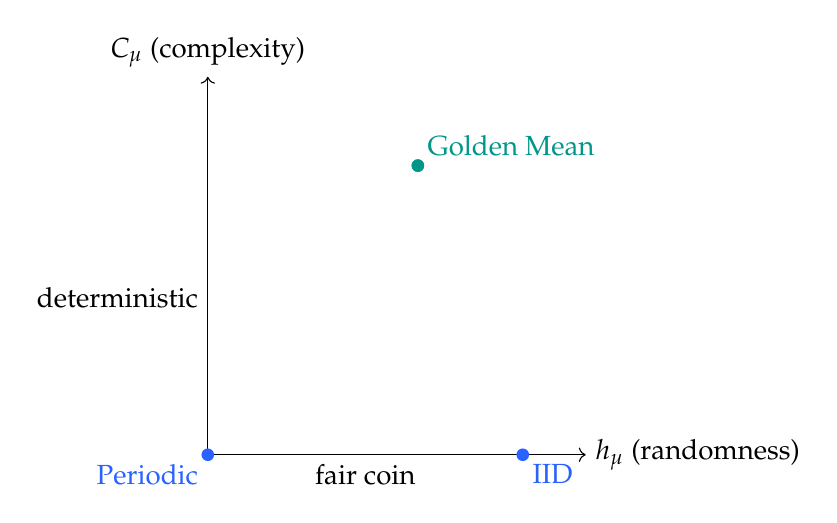
\begin{tikzpicture}[scale=4]
    % Axes
    \draw[->] (0,0) -- (1.2,0) node[right] {$\hmu$ (randomness)};
    \draw[->] (0,0) -- (0,1.2) node[above] {$\Cmu$ (complexity)};

    % Points
    \fill[emicblue] (0,0) circle (0.02) node[below left] {Periodic};
    \fill[emicblue] (1,0) circle (0.02) node[below right] {IID};
    \fill[emicgreen] (0.667,0.918) circle (0.02) node[above right] {Golden Mean};
    \fill[emicgreen] (0.667,0.918) circle (0.02);

    % Labels
    \node[anchor=north] at (0.5,0) {fair coin};
    \node[anchor=east] at (0,0.5) {deterministic};
\end{tikzpicture}
\end{center}

\begin{itemize}
    \item \textbf{Bottom-left} ($\hmu = 0, \Cmu = 0$): Constant sequences (no randomness, no structure)
    \item \textbf{Bottom-right} ($\hmu = 1, \Cmu = 0$): IID fair coin (maximum randomness, no structure)
    \item \textbf{Middle}: Interesting processes with both structure and randomness
\end{itemize}

The ``edge of chaos'' lives in the middle---complex enough to be interesting, structured enough to be predictable.

%%%%%%%%%%%%%%%%%%%%%%%%%%%%%%%%%%%%%%%%%%%%%%%%%%%%%%%%%%%%%%%%%%%%%
\part{\texorpdfstring{Inference: From Data to $\eps$-Machine}{Inference: From Data to Epsilon-Machine}}
%%%%%%%%%%%%%%%%%%%%%%%%%%%%%%%%%%%%%%%%%%%%%%%%%%%%%%%%%%%%%%%%%%%%%

% ===================================================================
\section{The CSSR Algorithm}
\label{sec:cssr}
% ===================================================================

\textbf{CSSR} (Causal State Splitting Reconstruction) is the standard algorithm for inferring $\eps$-machines from data~\cite{shalizi2004algorithm}.

\subsection{The Idea}

\begin{enumerate}
    \item Start with a single state containing all histories
    \item Test if histories in a state are ``homogeneous'' (same predictive distribution)
    \item If not, \textbf{split} the state based on predictive differences
    \item Iterate until all states are homogeneous
\end{enumerate}

\subsection{Homogeneity Testing}

Two histories are in the same state only if their next-symbol distributions are statistically indistinguishable. CSSR uses a $\chi^2$ test or similar.

\subsection{The Over-Splitting Problem}

\begin{warning}[title=CSSR's Achilles Heel]
CSSR can \textbf{over-split} states when data is limited. If two histories happen to have different empirical distributions due to sampling noise, CSSR may incorrectly split them into separate states---even when they belong to the same true causal state.
\end{warning}

\paragraph{Why does over-splitting happen?}
Consider the Golden Mean process with its 2 true states. Suppose we observe:
\begin{itemize}[nosep]
    \item History ``01'': followed by 0 in 48\% of cases, 1 in 52\%
    \item History ``11'': followed by 0 in 52\% of cases, 1 in 48\%
\end{itemize}

The true distribution for both is 50/50, but sampling noise created a difference. If our significance threshold is too strict, CSSR's $\chi^2$ test rejects the hypothesis that they're equal---and we get 3+ states instead of 2.

\paragraph{Consequences of over-splitting.}
\begin{itemize}[nosep]
    \item \textbf{Inflated complexity}: $\Cmu$ is overestimated
    \item \textbf{Poor generalization}: The model overfits to training data
    \item \textbf{Spurious structure}: We ``discover'' patterns that don't exist
\end{itemize}

\paragraph{CSSR's mitigation strategies.}
CSSR includes heuristics to reduce over-splitting:
\begin{enumerate}[nosep]
    \item \textbf{Significance level}: Higher $\alpha$ (e.g., 0.05 vs 0.001) makes tests more lenient
    \item \textbf{State merging}: After splitting, attempt to merge states with similar distributions
    \item \textbf{More data}: With enough samples, empirical distributions converge to truth
\end{enumerate}

But these are heuristics, not guarantees. For a principled solution, we turn to spectral methods.

% ===================================================================
\section{Spectral Learning: A Linear Algebra Approach}
\label{sec:spectral}
% ===================================================================

\textbf{Spectral learning}~\cite{hsu2012spectral,boots2011closing} offers an elegant alternative to CSSR's hypothesis testing. Instead of iteratively splitting states, it recovers the model structure in one shot using linear algebra.

\subsection{The Key Insight: Hankel Matrices}

The central object is the \textbf{Hankel matrix} $H$, which organizes sequence probabilities:

\begin{equation}
    H_{ij} = P(\text{prefix } p_i, \text{suffix } s_j)
\end{equation}

where $p_i$ ranges over history strings and $s_j$ ranges over future strings.

\begin{example}[title=A Small Hankel Matrix]
For a binary alphabet with histories/futures up to length 2:
\[
H = \begin{pmatrix}
P(\epsilon, \epsilon) & P(\epsilon, 0) & P(\epsilon, 1) & P(\epsilon, 00) & \cdots \\
P(0, \epsilon) & P(0, 0) & P(0, 1) & P(0, 00) & \cdots \\
P(1, \epsilon) & P(1, 0) & P(1, 1) & P(1, 00) & \cdots \\
P(00, \epsilon) & P(00, 0) & P(00, 1) & P(00, 00) & \cdots \\
\vdots & \vdots & \vdots & \vdots & \ddots
\end{pmatrix}
\]
where $\epsilon$ is the empty string and $P(p, s) = P(\text{seeing } p \text{ then } s)$.
\end{example}

\subsection{The Rank Reveals the States}

Here's the magic: \textbf{the rank of $H$ equals the number of causal states!}

\begin{theorembox}[title=Hankel Rank Theorem]
For a stationary process generated by a minimal HMM with $k$ states:
\begin{equation}
    \text{rank}(H) = k
\end{equation}
\end{theorembox}

\paragraph{Why does this work?} The Hankel matrix can be factored as:
\begin{equation}
    H = \Omega \cdot D \cdot \Lambda^\top
\end{equation}
where:
\begin{itemize}[nosep]
    \item $\Omega$ (history $\to$ state): maps histories to state distributions
    \item $D$: diagonal matrix of stationary state probabilities
    \item $\Lambda$ (state $\to$ future): maps states to future distributions
\end{itemize}

Both $\Omega$ and $\Lambda$ have rank $k$ (the number of states), so their product has rank $\leq k$. For a minimal model, the rank is exactly $k$.

\subsection{The Algorithm}

Spectral learning proceeds as:

\begin{enumerate}
    \item \textbf{Estimate $H$}: Count substring frequencies from data
    \item \textbf{Compute SVD}: $H \approx U \Sigma V^\top$
    \item \textbf{Determine rank}: Find the ``elbow'' where singular values drop off
    \item \textbf{Extract model}: Recover transition matrices from the SVD factors
\end{enumerate}

\subsection{Why Spectral Methods Avoid Over-Splitting}

\begin{keyidea}
Spectral methods determine the number of states \textbf{globally} from the rank of $H$, not \textbf{locally} from pairwise tests between histories.
\end{keyidea}

\paragraph{The key advantages:}
\begin{itemize}
    \item \textbf{Noise averaging}: The Hankel matrix aggregates information from \emph{all} prefix-suffix pairs. Noise in individual entries averages out.
    \item \textbf{Rank stability}: Small perturbations to $H$ cause small perturbations to singular values. We can reliably identify large gaps in the spectrum.
    \item \textbf{No cascading errors}: CSSR's splits are sequential---early mistakes propagate. Spectral methods make one global decision.
    \item \textbf{Principled regularization}: We can use the singular value spectrum to balance model complexity against fit.
\end{itemize}

\begin{example}[title=Spectral vs CSSR on Noisy Data]
Consider 10,000 samples from the Golden Mean (2 true states):
\begin{itemize}[nosep]
    \item \textbf{CSSR} (significance=0.01): Often infers 3--4 states
    \item \textbf{Spectral}: Singular values are $[\sigma_1, \sigma_2, \sigma_3, \ldots] = [1.2, 0.8, 0.02, 0.01, \ldots]$

    Clear gap after 2 values $\Rightarrow$ correctly infers 2 states
\end{itemize}
\end{example}

\subsection{Using emic's Spectral Learning}

\begin{lstlisting}
from emic import Spectral, SpectralConfig
from emic.sources import GoldenMean

source = GoldenMean(p=0.5)
data = source.generate(10_000)  # Spectral is sample-efficient

# Default config uses adaptive parameters based on sample size
config = SpectralConfig()  # Automatically sets max_history, min_count
spectral = Spectral(config)
result = spectral.infer(data)

print(f"Inferred {result.machine.num_states} states")

# For expert control, parameters can be set explicitly:
# config = SpectralConfig(
#     max_history=10,        # Fixed history length (None = adaptive)
#     rank_threshold=0.001,  # Singular value cutoff (lower = fewer states)
#     rank=2,                # Or fix rank directly when known
#     min_count=5            # Minimum observations per history (None = adaptive)
# )
\end{lstlisting}

\subsection{Algorithm Comparison}

The following table summarizes the key trade-offs between all five inference
algorithms. Based on our benchmarks across diverse processes, we provide
practical guidance for algorithm selection.

\begin{center}
\small
\begin{tabular}{lccccc}
\toprule
\textbf{Property} & \textbf{CSSR} & \textbf{Spectral} & \textbf{CSM} & \textbf{NSD} & \textbf{BSI} \\
\midrule
Sample efficiency & Moderate & \textbf{High} & Moderate & Moderate & Low \\
Accuracy (N$\geq$1K) & 80\% & \textbf{98\%} & 45\% & 75\% & 25\% \\
Over-splitting risk & High & Low & Low & Low & N/A \\
Under-splitting risk & Low & Moderate & High & Moderate & High \\
Interpretability & Direct & Post-process & Direct & Low & Probabilistic \\
Unifilarity guarantee & Yes & No & No & No & No \\
Max states control & No & Via rank & No & Yes & Yes \\
\bottomrule
\end{tabular}
\end{center}

\begin{intuition}
\textbf{Recommendation}: Start with \textbf{Spectral} for most applications---it achieves
98\% accuracy at $N \geq 1000$ samples with adaptive defaults. Use \textbf{CSSR}
when you need guaranteed unifilarity. Use \textbf{NSD} or \textbf{BSI} when you need
to bound the number of states. Use \textbf{CSM} when you want hierarchical insights
into state structure.
\end{intuition}

\subsection{Using emic}

\begin{lstlisting}
from emic import CSSR, CSSRConfig
from emic.sources import GoldenMean

# Generate data
source = GoldenMean(p=0.5)
data = source.generate(100_000)

# Configure and run CSSR
config = CSSRConfig(max_history=5, significance=0.01)
cssr = CSSR(config)
result = cssr.infer(data)

print(f"Inferred {result.machine.num_states} states")
\end{lstlisting}

% ===================================================================
\section{Robustness to Observation Noise}
\label{sec:noise-robustness}
% ===================================================================

Real-world data is noisy. How do inference algorithms behave when observations are corrupted? We tested all five algorithms on the Golden Mean process with bit-flip noise at levels $\varepsilon \in [0, 0.5]$ (50 repetitions each, $N=10{,}000$ samples).

\begin{figure}[htbp]
\centering
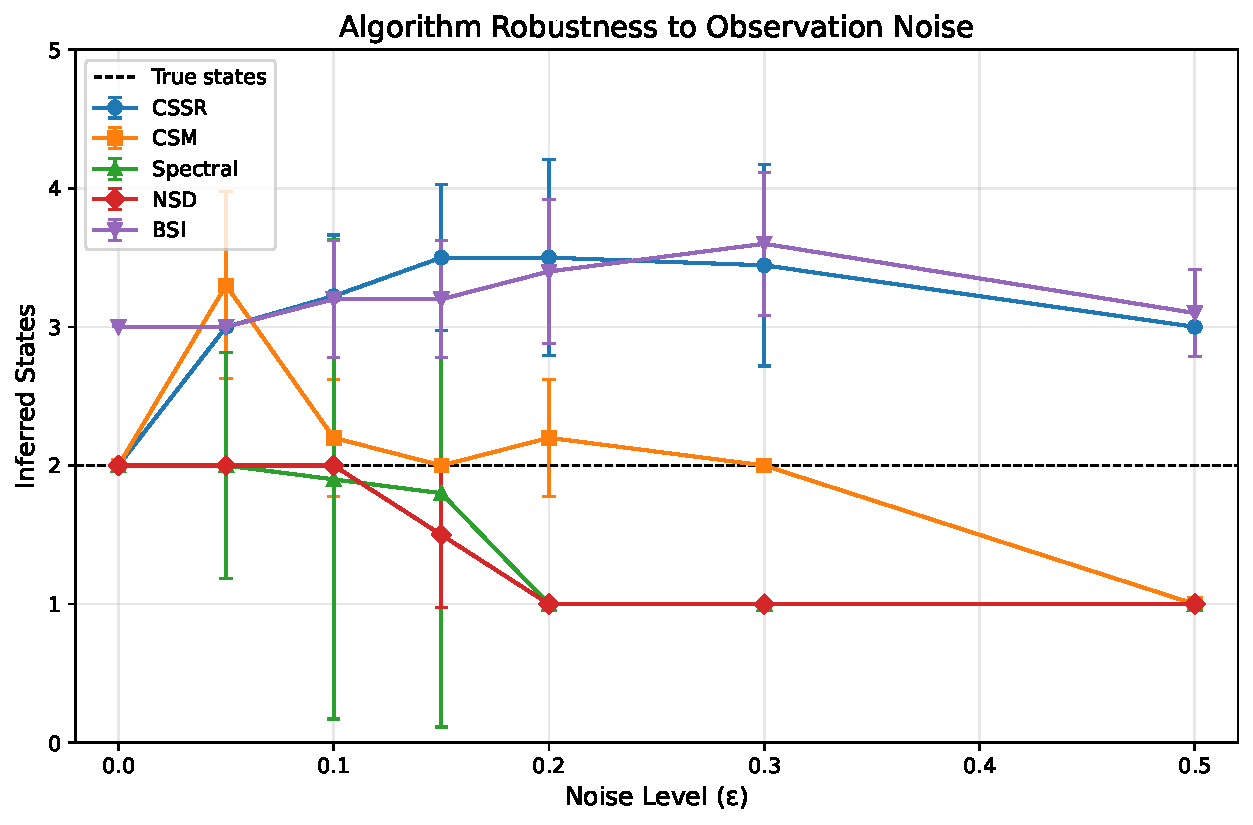
\includegraphics[width=0.85\textwidth]{figures/states_vs_noise.pdf}
\caption{Inferred states vs.\ noise level for the Golden Mean process (true states = 2). Error bars show $\pm 1$ standard deviation across 50 runs.}
\label{fig:noise-robustness}
\end{figure}

% Auto-generated from experiments/noise_robustness/analyze_noise.py
\begin{center}
\small
\begin{tabular}{lccccc}
\toprule
\textbf{Algorithm} & \textbf{$\varepsilon=0$} & \textbf{$\varepsilon=0.05$} & \textbf{$\varepsilon=0.1$} & \textbf{$\varepsilon=0.2$} & \textbf{$\varepsilon=0.5$} \\
\midrule
CSSR & 2.0$\pm$0.0 & 3.0$\pm$0.0 & 3.2$\pm$0.4 & 3.5$\pm$0.7 & 3.0$\pm$0.0 \\
CSM & 2.0$\pm$0.0 & 3.3$\pm$0.7 & 2.2$\pm$0.4 & 2.2$\pm$0.4 & 1.0$\pm$0.0 \\
Spectral & 2.0$\pm$0.0 & 2.0$\pm$0.8 & 1.9$\pm$1.7 & 1.0$\pm$0.0 & 1.0$\pm$0.0 \\
NSD & 2.0$\pm$0.0 & 2.0$\pm$0.0 & 2.0$\pm$0.0 & 1.0$\pm$0.0 & 1.0$\pm$0.0 \\
BSI & 3.0$\pm$0.0 & 3.0$\pm$0.0 & 3.2$\pm$0.4 & 3.4$\pm$0.5 & 3.1$\pm$0.3 \\
\bottomrule
\end{tabular}

\end{center}

\begin{intuition}
\textbf{Key findings}:
\begin{itemize}
    \item \textbf{CSSR} over-splits with noise, finding 3+ states at moderate noise levels
    \item \textbf{Spectral/NSD} under-split at high noise, collapsing to 1 state
    \item \textbf{CSM} shows bipolar behavior: over-splits at low noise, under-splits at high noise
    \item \textbf{BSI} consistently over-splits (even at $\varepsilon=0$), suggesting prior/hyperparameter tuning is needed
\end{itemize}
No algorithm is universally robust. For noisy data, cross-validate with multiple algorithms and be skeptical of results.
\end{intuition}

\section{The Bayesian Perspective}
\label{sec:bayesian}
% ===================================================================

CSSR takes a frequentist approach: test hypotheses about state equality. An alternative is \textbf{Bayesian Structural Inference (BSI)}, which provides full posterior distributions over model structures.

The Bayesian approach to inference is well-established in machine learning~\cite{bishop2006pattern}. For a general introduction to HMM inference, see Rabiner's tutorial~\cite{rabiner1989tutorial}.

\subsection{The Bayesian Setup}

Instead of testing, we compute:
\begin{equation}
    P(\text{structure} | \text{data}) \propto P(\text{data} | \text{structure}) \cdot P(\text{structure})
\end{equation}

\subsection{Dirichlet-Multinomial Framework}

For each state $\sigma$, we model the emission distribution with a Dirichlet prior:
\begin{equation}
    (\theta_0, \theta_1, \ldots) \sim \text{Dirichlet}(\alpha, \alpha, \ldots)
\end{equation}

The posterior after observing counts $(c_0, c_1, \ldots)$ is:
\begin{equation}
    \text{Dirichlet}(\alpha + c_0, \alpha + c_1, \ldots)
\end{equation}

\begin{keyidea}
The conjugacy of Dirichlet-Multinomial makes Bayesian updates easy: just add counts to prior pseudocounts!
\end{keyidea}

\subsection{Gibbs Sampling for State Assignments}

BSI uses Gibbs sampling to explore possible state assignments:

\begin{enumerate}
    \item Initialize: assign each history to a random state
    \item For each history $h$:
    \begin{itemize}
        \item Compute probability of $h$ belonging to each state (using Dirichlet-Multinomial)
        \item Sample a new assignment proportional to these probabilities
    \end{itemize}
    \item Repeat until convergence
\end{enumerate}

\subsection{Advantages of BSI}

\begin{itemize}
    \item \textbf{Uncertainty quantification}: Get posterior distributions, not point estimates
    \item \textbf{Model selection}: Compare models with different numbers of states
    \item \textbf{Regularization}: Priors prevent overfitting
    \item \textbf{Small data}: Works better with limited observations
\end{itemize}

\subsection{Using emic's BSI}

\begin{lstlisting}
from emic import BSI, BSIConfig
from emic.sources import GoldenMean

source = GoldenMean(p=0.5)
data = source.generate(10_000)

config = BSIConfig(
    max_states=5,
    alpha_prior=1.0,  # Symmetric Dirichlet
    n_samples=1000,
    burnin=200
)
bsi = BSI(config)
result = bsi.infer(data)

print(f"Inferred {result.machine.num_states} states")
\end{lstlisting}

% ===================================================================
\section{Causal State Merging (CSM)}
\label{sec:csm}
% ===================================================================

\textbf{Causal State Merging} (CSM) takes a bottom-up approach, in contrast
to CSSR's top-down splitting. Starting from the finest possible partition---where
each unique history of length $L$ defines its own state---CSM progressively
merges states whose predictive distributions are statistically indistinguishable.

\subsection{Algorithm Intuition}

\begin{enumerate}
    \item \textbf{Initialize}: Create one state per unique $L$-history.
    \item \textbf{Compute distances}: For each pair of states, measure how
          different their predictive distributions are.
    \item \textbf{Merge}: Combine the two closest states (if below threshold).
    \item \textbf{Repeat}: Continue until no pairs are close enough to merge.
\end{enumerate}

CSM naturally produces a hierarchical clustering (dendrogram) over states,
which can be useful for exploring the structure at different granularities.

\subsection{Distance Metrics}

CSM supports several metrics for comparing predictive distributions:

\begin{itemize}
    \item \textbf{KL divergence}: $D_{\text{KL}}(P \| Q) = \sum_x P(x) \log \frac{P(x)}{Q(x)}$
    \item \textbf{Hellinger}: $H(P, Q) = \frac{1}{\sqrt{2}} \sqrt{\sum_x (\sqrt{P(x)} - \sqrt{Q(x)})^2}$
    \item \textbf{Total variation}: $\text{TV}(P, Q) = \frac{1}{2} \sum_x |P(x) - Q(x)|$
    \item \textbf{Chi-squared}: Useful for hypothesis testing interpretation
\end{itemize}

\subsection{Using emic's CSM}

\begin{lstlisting}
from emic import CSM, CSMConfig
from emic.sources import GoldenMean

source = GoldenMean(p=0.5)
data = source.generate(50_000)

config = CSMConfig(
    history_length=5,       # Initial partition granularity
    merge_threshold=0.05,   # Distance threshold for merging
    distance_metric='kl',   # KL divergence (or 'hellinger', 'tv', 'chi2')
    min_count=5             # Minimum observations per history
)
csm = CSM(config)
result = csm.infer(data)

print(f"Inferred {result.machine.num_states} states")
\end{lstlisting}

\subsection{Trade-offs}

\begin{itemize}
    \item \textbf{Pros}: Avoids over-splitting; produces interpretable hierarchies;
          robust when data is noisy.
    \item \textbf{Cons}: May under-split if threshold is too aggressive;
          computational cost grows with number of unique histories;
          requires choosing history length upfront.
\end{itemize}

% ===================================================================
\section{Neural State Discovery (NSD)}
\label{sec:nsd}
% ===================================================================

\textbf{Neural State Discovery} (NSD) uses machine learning techniques to
learn state representations. Rather than relying on explicit statistical
tests, NSD learns embeddings of histories and clusters them to discover
causal states.

\subsection{Algorithm Intuition}

\begin{enumerate}
    \item \textbf{Embed}: Map each history to a vector representation.
    \item \textbf{Cluster}: Group similar embeddings using k-means or similar.
    \item \textbf{Extract}: Build the $\eps$-machine from the discovered clusters.
\end{enumerate}

NSD is particularly useful when:
\begin{itemize}
    \item The process has complex, high-dimensional structure
    \item You want to bound the number of states explicitly
    \item Traditional statistical tests are unreliable due to limited data
\end{itemize}

\subsection{Using emic's NSD}

\begin{lstlisting}
from emic import NSD, NSDConfig
from emic.sources import GoldenMean

source = GoldenMean(p=0.5)
data = source.generate(20_000)

config = NSDConfig(
    max_states=5,           # Upper bound on states
    history_length=10,      # History window for embeddings
    embedding_dim=16,       # Dimensionality of embeddings
    n_iterations=100,       # Clustering iterations
    seed=42                 # For reproducibility
)
nsd = NSD(config)
result = nsd.infer(data)

print(f"Inferred {result.machine.num_states} states")
\end{lstlisting}

\subsection{Trade-offs}

\begin{itemize}
    \item \textbf{Pros}: Explicit control over maximum states; can handle
          complex patterns; reproducible with fixed seed.
    \item \textbf{Cons}: Less interpretable than CSSR/CSM; requires
          parameter tuning; may not find the minimal model.
\end{itemize}

%%%%%%%%%%%%%%%%%%%%%%%%%%%%%%%%%%%%%%%%%%%%%%%%%%%%%%%%%%%%%%%%%%%%%
\part{Worked Examples}
%%%%%%%%%%%%%%%%%%%%%%%%%%%%%%%%%%%%%%%%%%%%%%%%%%%%%%%%%%%%%%%%%%%%%

% ===================================================================
\section{Example 1: The Biased Coin}
\label{sec:example-coin}
% ===================================================================

The simplest process: independent flips of a biased coin.

\begin{itemize}
    \item \textbf{States}: 1 (all histories are equivalent)
    \item \textbf{$\Cmu$}: 0 bits (no memory needed)
    \item \textbf{$\hmu$}: $-p \log_2 p - (1-p) \log_2 (1-p)$ bits
\end{itemize}

\begin{lstlisting}
from emic import BiasedCoin, CSSR
from emic.analysis import statistical_complexity, entropy_rate

source = BiasedCoin(p=0.7)
data = source.generate(50_000)
machine = CSSR().infer(data).machine

print(f"States: {machine.num_states}")  # 1
print(f"Cmu: {statistical_complexity(machine):.3f}")  # 0.000
print(f"hmu: {entropy_rate(machine):.3f}")  # 0.881
\end{lstlisting}

% ===================================================================
\section{Example 2: The Golden Mean Process}
\label{sec:example-golden-mean}
% ===================================================================

Binary sequences where 0 must be followed by 1.

\begin{center}
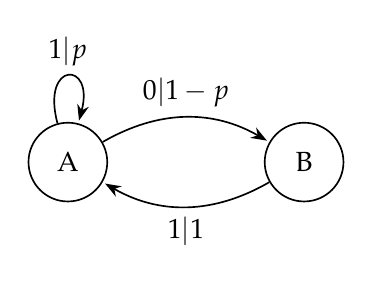
\begin{tikzpicture}[->,>=Stealth,shorten >=1pt,auto,node distance=3cm,
                    semithick,every state/.style={minimum size=1cm}]
    \node[state] (A) {A};
    \node[state] (B) [right of=A] {B};

    \path (A) edge [loop above] node {$1|p$} (A)
          (A) edge [bend left]  node {$0|1-p$} (B)
          (B) edge [bend left]  node {$1|1$} (A);
\end{tikzpicture}
\end{center}

For $p = 0.5$:
\begin{itemize}
    \item \textbf{States}: 2
    \item \textbf{Stationary distribution}: $\pi(A) = 2/3$, $\pi(B) = 1/3$
    \item \textbf{$\Cmu$}: $\approx 0.918$ bits
    \item \textbf{$\hmu$}: $= 2/3$ bits
\end{itemize}

% ===================================================================
\section{Example 3: The Even Process}
\label{sec:example-even}
% ===================================================================

Binary sequences where 1s come in runs of even length.

\begin{center}
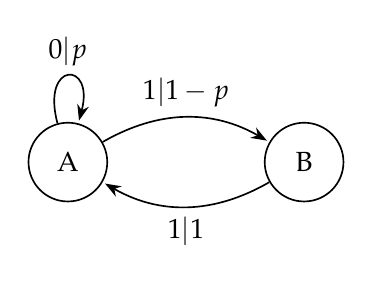
\begin{tikzpicture}[->,>=Stealth,shorten >=1pt,auto,node distance=3cm,
                    semithick,every state/.style={minimum size=1cm}]
    \node[state] (A) {A};
    \node[state] (B) [right of=A] {B};

    \path (A) edge [loop above] node {$0|p$} (A)
          (A) edge [bend left]  node {$1|1-p$} (B)
          (B) edge [bend left]  node {$1|1$} (A);
\end{tikzpicture}
\end{center}

Interestingly, for $p = 0.5$, the Even Process has the same $\Cmu$ and $\hmu$ as the Golden Mean---they're ``complexity twins''!

% ===================================================================
\section{Example 4: Periodic Processes}
\label{sec:example-periodic}
% ===================================================================

A period-$n$ process cycles through $n$ states deterministically.

\begin{itemize}
    \item \textbf{States}: $n$
    \item \textbf{$\Cmu$}: $\log_2 n$ bits
    \item \textbf{$\hmu$}: 0 bits (completely predictable)
\end{itemize}

\begin{lstlisting}
from emic import Periodic, CSSR
from emic.analysis import statistical_complexity, entropy_rate

for n in [2, 3, 5, 10]:
    source = Periodic(period=n)
    data = source.generate(10_000)
    machine = CSSR().infer(data).machine
    print(f"Period {n}: Cmu={statistical_complexity(machine):.3f}, "
          f"hmu={entropy_rate(machine):.3f}")
\end{lstlisting}

Output:
\begin{verbatim}
Period 2: Cmu=1.000, hmu=0.000
Period 3: Cmu=1.585, hmu=0.000
Period 5: Cmu=2.322, hmu=0.000
Period 10: Cmu=3.322, hmu=0.000
\end{verbatim}

%%%%%%%%%%%%%%%%%%%%%%%%%%%%%%%%%%%%%%%%%%%%%%%%%%%%%%%%%%%%%%%%%%%%%
\part{Going Further}
%%%%%%%%%%%%%%%%%%%%%%%%%%%%%%%%%%%%%%%%%%%%%%%%%%%%%%%%%%%%%%%%%%%%%

% ===================================================================
\section{Connections to Other Frameworks}
\label{sec:connections}
% ===================================================================

\subsection{Hidden Markov Models}

The $\eps$-machine is a special kind of HMM:
\begin{itemize}
    \item HMMs in general are not unifilar
    \item The $\eps$-machine is the \emph{minimal unifilar} HMM
    \item Standard HMM learning (Baum-Welch) doesn't find the $\eps$-machine
\end{itemize}

\subsection{Minimum Description Length}

MDL asks: what's the shortest program to describe the data? Computational Mechanics asks: what's the minimal memory for optimal prediction? These are related but distinct.

\subsection{Kolmogorov Complexity}

Kolmogorov complexity is the length of the shortest program to produce a \emph{single} sequence. It's uncomputable and defined for individuals. $\Cmu$ is computable and defined for ensembles (distributions).

% ===================================================================
\section{Open Questions}
\label{sec:open-questions}
% ===================================================================

\begin{enumerate}
    \item \textbf{Infinite-state processes}: What happens when $|\calS| = \infty$?
    \item \textbf{Continuous processes}: How to extend to continuous alphabets/time?
    \item \textbf{Quantum processes}: Can quantum mechanics reduce $\Cmu$?
    \item \textbf{Higher-order structure}: When HMMs fail, what comes next?
\end{enumerate}

% ===================================================================
\section{Further Reading}
\label{sec:further-reading}
% ===================================================================

\begin{itemize}
    \item \textbf{The foundational paper}: Shalizi \& Crutchfield~\cite{shalizi2001computational}, ``Computational Mechanics: Pattern and Prediction, Structure and Simplicity''
    \item \textbf{Philosophical context}: Crutchfield~\cite{crutchfield1994calculi}, ``The Calculi of Emergence''
    \item \textbf{The CSSR algorithm}: Shalizi \& Klinkner~\cite{shalizi2004algorithm}
    \item \textbf{Information theory}: Shannon~\cite{shannon1948mathematical}, Cover \& Thomas~\cite{cover2006elements}
    \item \textbf{Quantum extensions}: Gu et al.~\cite{gu2012quantum}, Thompson et al.~\cite{thompson2018causal}
    \item \textbf{Software}: The \texttt{emic} Python library~\cite{emic2026}
\end{itemize}

% ===================================================================
% BIBLIOGRAPHY
% ===================================================================
\bibliographystyle{plain}
\bibliography{../shared/bibliography/references}

\end{document}
